%% ----------------------------------------------------------------
%% Thesis.tex -- MAIN FILE (the one that you compile with LaTeX)
%% ---------------------------------------------------------------- 

% Set up the document
\documentclass[a4paper, 11pt, oneside]{Thesis}  % Use the "Thesis" style, based on the ECS Thesis style by Steve Gunn
\graphicspath{{Figures/}}  % Location of the graphics files (set up for graphics to be in PDF format)
\usepackage{amsmath, amsfonts, amssymb, amsthm, epsfig, epstopdf, titling, url, array}
% Include any extra LaTeX packages required
\usepackage[square, numbers, comma, sort&compress]{natbib}  % Use the "Natbib" style for the references in the Bibliography
\usepackage{verbatim}  % Needed for the "comment" environment to make LaTeX comments
\usepackage{vector}  % Allows "\bvec{}" and "\buvec{}" for "blackboard" style bold vectors in maths
\hypersetup{urlcolor=blue, colorlinks=true}  % Colours hyperlinks in blue, but this can be distracting if there are many links.

\theoremstyle{plain}
\newtheorem{thm}{Theorem}[section]
\newtheorem{lem}[thm]{Lemma}
\newtheorem{prop}[thm]{Proposition}
\newtheorem*{cor}{Corollary}

\theoremstyle{definition}
\newtheorem{defn}{Definition}[section]
\newtheorem{conj}{Conjecture}[section]
\newtheorem{exmp}{Example}[section]

\theoremstyle{remark}
\newtheorem*{rem}{Remark}
\newtheorem*{note}{Note}


%% ----------------------------------------------------------------
\begin{document}
\frontmatter      % Begin Roman style (i, ii, iii, iv...) page numbering

% Set up the Title Page
\title  {Machine Learning on Forex Carry forecasting with Economic features}
\authors  {\texorpdfstring
            {\href{r02323025@ntu.edu.tw}{Eugene-Yuan Kou}}
            {Author Name}
            }
\addresses  {\groupname\\\deptname\\\univname}  % Do not change this here, instead these must be set in the "Thesis.cls" file, please look through it instead
\date       {\today}
\subject    {}
\keywords   {}

\maketitle
%% ----------------------------------------------------------------

\setstretch{1.3}  % It is better to have smaller font and larger line spacing than the other way round

% Define the page headers using the FancyHdr package and set up for one-sided printing
\fancyhead{}  % Clears all page headers and footers
\rhead{\thepage}  % Sets the right side header to show the page number
\lhead{}  % Clears the left side page header

\pagestyle{fancy}  % Finally, use the "fancy" page style to implement the FancyHdr headers

%% ----------------------------------------------------------------
% Declaration Page required for the Thesis, your institution may give you a different text to place here
\Declaration{

\addtocontents{toc}{\vspace{1em}}  % Add a gap in the Contents, for aesthetics

I, Eugene-Yuan Kou, declare that this thesis titled, `THESIS TITLE' and the work presented in it are my own. I confirm that:

\begin{itemize} 
\item[\tiny{$\blacksquare$}] This work was done wholly or mainly while in candidature for a research degree at this University.
 
\item[\tiny{$\blacksquare$}] Where any part of this thesis has previously been submitted for a degree or any other qualification at this University or any other institution, this has been clearly stated.
 
\item[\tiny{$\blacksquare$}] Where I have consulted the published work of others, this is always clearly attributed.
 
\item[\tiny{$\blacksquare$}] Where I have quoted from the work of others, the source is always given. With the exception of such quotations, this thesis is entirely my own work.
 
\item[\tiny{$\blacksquare$}] I have acknowledged all main sources of help.
 
\item[\tiny{$\blacksquare$}] Where the thesis is based on work done by myself jointly with others, I have made clear exactly what was done by others and what I have contributed myself.
\\
\end{itemize}
 
 
Signed:\\
\rule[1em]{25em}{0.5pt}  % This prints a line for the signature
 
Date:\\
\rule[1em]{25em}{0.5pt}  % This prints a line to write the date
}
\clearpage  % Declaration ended, now start a new page

%% ----------------------------------------------------------------
% The "Funny Quote Page"
\pagestyle{empty}  % No headers or footers for the following pages

\null\vfill
% Now comes the "Funny Quote", written in italics
\textit{``Write a funny quote here.''}

\begin{flushright}
If the quote is taken from someone, their name goes here
\end{flushright}

\vfill\vfill\vfill\vfill\vfill\vfill\null
\clearpage  % Funny Quote page ended, start a new page
%% ----------------------------------------------------------------

% The Abstract Page
\addtotoc{Abstract}  % Add the "Abstract" page entry to the Contents
\abstract{
\addtocontents{toc}{\vspace{1em}}  % Add a gap in the Contents, for aesthetics

The Thesis Abstract is written here (and usually kept to just this page). The page is kept centered vertically so can expand into the blank space above the title too\ldots

}

\clearpage  % Abstract ended, start a new page
%% ----------------------------------------------------------------

\setstretch{1.3}  % Reset the line-spacing to 1.3 for body text (if it has changed)

% The Acknowledgements page, for thanking everyone
\acknowledgements{
\addtocontents{toc}{\vspace{1em}}  % Add a gap in the Contents, for aesthetics

The acknowledgements and the people to thank go here, don't forget to include your project advisor\ldots

}
\clearpage  % End of the Acknowledgements
%% ----------------------------------------------------------------

\pagestyle{fancy}  %The page style headers have been "empty" all this time, now use the "fancy" headers as defined before to bring them back


%% ----------------------------------------------------------------
\lhead{\emph{Contents}}  % Set the left side page header to "Contents"
\tableofcontents  % Write out the Table of Contents

%% ----------------------------------------------------------------
\lhead{\emph{List of Figures}}  % Set the left side page header to "List if Figures"
\listoffigures  % Write out the List of Figures

%% ----------------------------------------------------------------
\lhead{\emph{List of Tables}}  % Set the left side page header to "List of Tables"
\listoftables  % Write out the List of Tables

%% ----------------------------------------------------------------
\setstretch{1.5}  % Set the line spacing to 1.5, this makes the following tables easier to read
\clearpage  % Start a new page
\lhead{\emph{Abbreviations}}  % Set the left side page header to "Abbreviations"
\listofsymbols{ll}  % Include a list of Abbreviations (a table of two columns)
{
% \textbf{Acronym} & \textbf{W}hat (it) \textbf{S}tands \textbf{F}or \\
\textbf{LAH} & \textbf{L}ist \textbf{A}bbreviations \textbf{H}ere \\

}

%% ----------------------------------------------------------------
\clearpage  % Start a new page
\lhead{\emph{Physical Constants}}  % Set the left side page header to "Physical Constants"
\listofconstants{lrcl}  % Include a list of Physical Constants (a four column table)
{
% Constant Name & Symbol & = & Constant Value (with units) \\
Speed of Light & $c$ & $=$ & $2.997\ 924\ 58\times10^{8}\ \mbox{ms}^{-\mbox{s}}$ (exact)\\

}

%% ----------------------------------------------------------------
\clearpage  %Start a new page
\lhead{\emph{Symbols}}  % Set the left side page header to "Symbols"
\listofnomenclature{lll}  % Include a list of Symbols (a three column table)
{
% symbol & name & unit \\
$a$ & distance & m \\
$P$ & power & W (Js$^{-1}$) \\
& & \\ % Gap to separate the Roman symbols from the Greek
$\omega$ & angular frequency & rads$^{-1}$ \\
}
%% ----------------------------------------------------------------
% End of the pre-able, contents and lists of things
% Begin the Dedication page

\setstretch{1.3}  % Return the line spacing back to 1.3

\pagestyle{empty}  % Page style needs to be empty for this page
\dedicatory{For/Dedicated to/To my\ldots}

\addtocontents{toc}{\vspace{2em}}  % Add a gap in the Contents, for aesthetics


%% ----------------------------------------------------------------
\mainmatter	  % Begin normal, numeric (1,2,3...) page numbering
\pagestyle{fancy}  % Return the page headers back to the "fancy" style

% Include the chapters of the thesis, as separate files
% Just uncomment the lines as you write the chapters

\chapter{Introduction}

    We first introduce some building blocks of our model, consisting Support Vector Machine(SVM), Multi-layer Peceptron
(MLP), Random Forest, Restricted Boltzmann Machine (RBM), Conditional Restricted Boltzmann Machine ,and Hyper Model. A brief overlook of these models, we can divide these models in to two categories, supervised learning and unsupervised learning. Supervised learning is just like how our teachers and dear supervisors teach us, giving us some examples, which are "labeled" by them, and we learn from the examples, however unsupervised learning is like 
\section{Abstract}

Quisque tristique urna in lorem laoreet at laoreet quam congue. Donec dolor turpis, blandit non imperdiet aliquet, blandit et felis. In lorem nisi, pretium sit amet vestibulum sed, tempus et sem. Proin non ante turpis. Nulla imperdiet fringilla convallis. Vivamus vel bibendum nisl. Pellentesque justo lectus, molestie vel luctus sed, lobortis in libero. Nulla facilisi. Aliquam erat volutpat. Suspendisse vitae nunc nunc. Sed aliquet est suscipit sapien rhoncus non adipiscing nibh consequat. Aliquam metus urna, faucibus eu vulputate non, luctus eu justo.

\subsection{A Subsection}

Donec urna leo, vulputate vitae porta eu, vehicula blandit libero. Phasellus eget massa et leo condimentum mollis. Nullam molestie, justo at pellentesque vulputate, sapien velit ornare diam, nec gravida lacus augue non diam. Integer mattis lacus id libero ultrices sit amet mollis neque molestie. Integer ut leo eget mi volutpat congue. Vivamus sodales, turpis id venenatis placerat, tellus purus adipiscing magna, eu aliquam nibh dolor id nibh. Pellentesque habitant morbi tristique senectus et netus et malesuada fames ac turpis egestas. Sed cursus convallis quam nec vehicula. Sed vulputate neque eget odio fringilla ac sodales urna feugiat.

\section{Another Section}

Phasellus nisi quam, volutpat non ullamcorper eget, congue fringilla leo. Cras et erat et nibh placerat commodo id ornare est. Nulla facilisi. Aenean pulvinar scelerisque eros eget interdum. Nunc pulvinar magna ut felis varius in hendrerit dolor accumsan. Nunc pellentesque magna quis magna bibendum non laoreet erat tincidunt. Nulla facilisi.

Duis eget massa sem, gravida interdum ipsum. Nulla nunc nisl, hendrerit sit amet commodo vel, varius id tellus. Lorem ipsum dolor sit amet, consectetur adipiscing elit. Nunc ac dolor est. Suspendisse ultrices tincidunt metus eget accumsan. Nullam facilisis, justo vitae convallis sollicitudin, eros augue malesuada metus, nec sagittis diam nibh ut sapien. Duis blandit lectus vitae lorem aliquam nec euismod nisi volutpat. Vestibulum ornare dictum tortor, at faucibus justo tempor non. Nulla facilisi. Cras non massa nunc, eget euismod purus. Nunc metus ipsum, euismod a consectetur vel, hendrerit nec nunc. % Introduction

\chapter{Lecture Review}

    We first introduce building blocks of our model, consisting Support Vector Machine(SVM), Multi-layer Peceptron
(MLP), Random Forest, Restricted Boltzmann Machine (RBM), Conditional Restricted Boltzmann Machine, and Hyper Model. A brief overview of these models, we can divide these models in to two categories, supervised learning and unsupervised learning. Supervised learning is just like how teachers and dear supervisors teach us, giving us some examples, which are "labeled" by them, and we learn from the examples, however unsupervised learning is teachers give us a criteria to identify different objects, and we use the criteria to learn.



\section{A brief theoretical look into Machine Learning}
    A general issue Machine Learning models want to resolve is how well we can approximate the true generative function $f:\mathbb{X}\rightarrow\mathbb{Y} $, which generates observable data.
   
    For instance, as an economist, we are interested in forecasting future GDP, or other economic indices. Assume that $GDP_{t+1} =f(C_{t})$ is the truth, and we want to use our algorithm to choose $g(x)$ to approximate our target function $f(x)$, given the data $(\mathbb{x_{n}},\mathbb{y_{n}}) $ generated by the target function $f(x)$.% general model setup
%place the image

When we have the general setup of machine learning models, % what's model learned? how we get g(x)


Since we got the optimal $g(x)$ from our hypothesis set$\mathbb{H}$, how we assessment whether we have 'learned' from the data, or we just memorizing the labels in our data set.% how we evaluate the model

\clearpage
\subsection*{Model Complexity}
\subsubsection*{VC dimension}
Now we introduce the concept of VC dimension.
VC dimension (for Vapnik Chervonenkis dimension) (Vapnik and Chervonenkis (1968, 1971), Vapnik (1979)) measures the capacity of a hypothesis space. Capacity is a measure of complexity and measures the expressive power, richness or flexibility of a set of functions by assessing how wiggly its members can be.

\begin{defn}
The Vapnik-Chervonenkis dimension of a hypothesis set $\mathcal{}{H}$, denoted by $d_{vc}(\mathcal{H})$ or simply $d_{vc}$, is the largest value of $\mathcal{N}$ for which $\mathcal{m_{\mathbb{H}}}(\mathcal{f(N)})= 2^{N}$. for all $\mathcal{N}$ then $d_{vc}=\infty$

\end{defn}
%
For example, assume $\mathcal{H}$ is a hypothesis set which is linear separation model(use a line to separate data), we are given pairs of ${x_{n}, y_{n}} $, and $ x_{n} \in \mathcal{R^2}$. How many different binary combinations can we assign to the data set?

\begin{center}
{
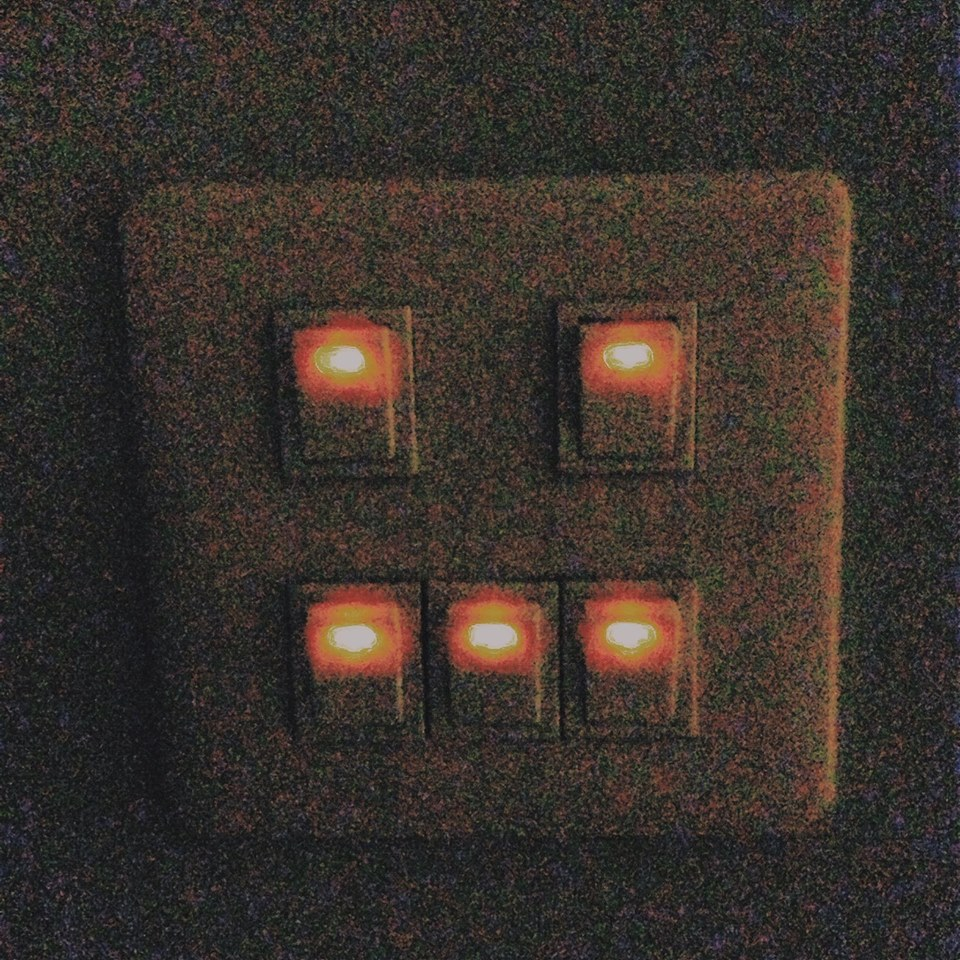
\includegraphics[width=7cm]{OOO}
}
\end{center}

%----- end VC dimension
\subsection*{Penalty for Model complexity}
Now we fuse above concepts together explaining the core philosophy of our modeling.
%----what is E_out ? E_val?


\subsection*{Cross Validation\& Model Selection}

\section{Supervised Learning}

\subsection{Support Vector Machine}

Cortes and Vapnik, Support Vector Machine(1995) is a discriminative model. We can write our problem into a general form.
$$ y = g(\sum^{K}_{i=1}{x_{i}}) \quad \textrm{and} \quad K \in \mathbb{R}$$
For basic model, $y \in \{-1, +1\}$  and $\ x_{i} \in \mathbb{R^{K}}$.
The formula shows SVMs can be easily applied on the regression model which we are familiar with. To introduce SVM we first introduce Hard-Margin Support Vector Machine(HmSVM).
\clearpage

The model can be written informally as follow.

$$\large{\max_{\mathbb{W}}} \ margin(\mathbb{W})$$
$$ s.t\ margin(\mathbb{W})=\min_{n=1...N} Distance(\mathbb{x_{n}},\mathbb{W})$$
$$ and\ \forall \ n \ y_{i}(\mathbb{w}^Tx_{n})>0$$
The maximization problem is to find the 'fattest' tube to perfectly separate our data, assuming the data set is separable(so called hard margin).
More clearly to illustrate SVM is to use graph, we have a data set which is already labeled in +1, and -1, ploted below.\\

\begin{center}
{
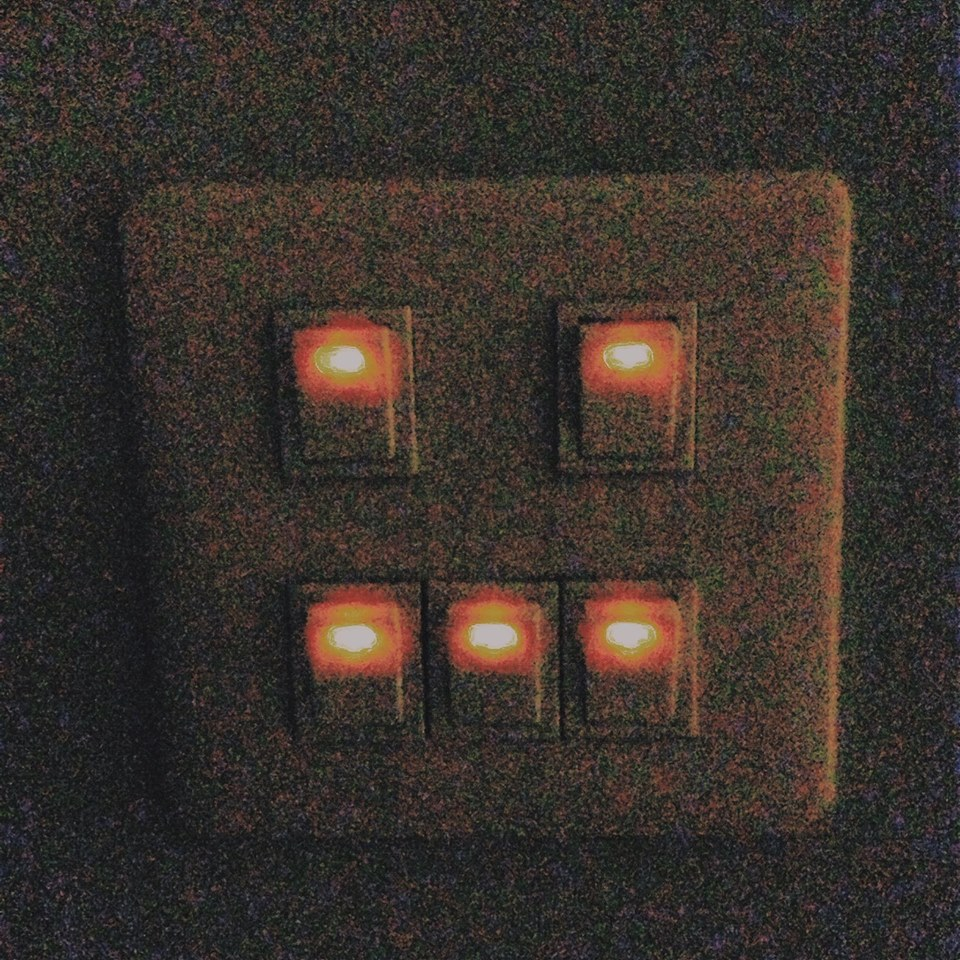
\includegraphics[width=7cm]{OOO}
}
\end{center}
The solution of hard-margin SVM is the red-colored tube which is the "fattest" from all potential candidates which can classify all training data.

As you can see from (1), hard-margin SVM does not assume any underlying distribution of our data set, but only the assumption of separability of our data set. However this condition can be easily loose by putting an bias term $\zeta$ 

%\subsubsection{Prime Problem}
More formal form of hard margin SVM is to rewrite the problem into quadratic form.

\subsubsection{Dual Problem}

More formal form of hard margin SVM is to rewrite the problem into quadratic form.

\subsubsection*{Kernel Transformation}
\subsubsection*{Poly Nominal Kernel}
\subsubsection*{Radial Basis Function Kernel}
\subsubsection*{Support Vectors}
Sparse solution


\subsection{Multi-layer Perceptron}
\subsubsection*{L1 and L2 regularization}

\subsection{Random Forest}
\subsubsection{Decision Tree}
\subsubsection*{Bagging}
\subsubsection*{Model Selection}
 % Background Theory 

\chapter{Experiment Design}

    we have conducted two experiments in this paper. First we are curious about whether the economics variables can predict the intra-day data of currency market, also gives a very beginning look of innovations methods applying on our problem.
    Second we apply our model on Forex carry strategy, which only put a lot of attention on the tomorrow's currency moment, and inherent the experience from our previous experiment to improve our model.


\section{Data Description}

For our first experiment we use one-month historical currency data in million-second based, and Wharton Research Data Services Fama-French, Coild-oil in daily based.

%https://pepperstone.com/mt4-forex-trading/mt4-tick-chart-history-data.php
%http://research.stlouisfed.org/fred2/series/DCOILWTICO
\begin{enumerate}
\item{GBP/JPY: tick-by-tick data in million-seconds for 2014-11}
\item{Crude Oil Prices: West Texas Intermediate (WTI) in daily frequency obtain from 1986-2014}
\item{Fama French \& Liquidity Factors: in daily frequency
from 2005-01-01 to 2015-03-31}
\item{The CBOE (Chicago Board Options Exchange) Volatility Index in daily frenquency}
\item{Current exchange rate Gold (XAU) to US DOLLAR (USD): tick-by-tick data in million-sec frequency for 2014-11}
\end{enumerate}
\newpage

    Since there are no representative papers support which economic factors are promising for forecasting exchange rate movement, or Forex carry daily return movement. We carry out an exploratory experiment to give a very look into our problem, which economic factors could give us a glance of future.
    
% Explain our data sets
    
    The only promising forecasting factor is currency forward. Financial theory suggests that under no arbitrage condition, the relation between forward rate and future exchange rate can be written as follow.

    For more deeply concern is that we apply the same concept from the paper[], using risk metric as independent variables to predict the future daily return movement of the portfolio.
    
    We also do some simple descriptive statistics on our data set. The result are as follow.
    

\begin{enumerate}
\item{}
\end{enumerate}


\subsection{Experiment 1}
    We ask a general question to our data set. The question can be written as follow.

$$ y_{t} = x_{t} + y_{t-1} +y_{t-2} + y_{i-3} +y_{i-4}+ y_{i-5}+
y_{i-6}$$

\subsection{Labeling}
    In the prototyping phrase we found that labeling plays a crucial part in model prediction. 
We present two types of labeling, first.

\subsection{Information Criteria}

    For this paper we want to test whether our features are containing crucial information helping us to make prediction.
We define the Information Criteria for our model as follow:
\newpage

\begin{defn}
Information content of factors\\
Information information content of factors of a model is that how much we can do better than we know nothing.
\end{defn}

\[
\mathbf{I}(\mathbf{x_t}) = \frac{\{ Error_{out} \mid g(\mathbf{x_{t}}) - Error_{out} \mid g(\mathbf{\epsilon_{t}})\}_{+}}
{Error_{out} \mid g(\mathbf{x_{t}},y_{t+1})}
\]

    The $ \mathbf{x_{t}} $ in our experiment is the economic feature of the market, $ g(x) $ is the approximation function, $ g(x) \in \mathcal{H}$, which we use our algorithm to find out, and $ g(\mathbf{x}, y_{t+1}) $ is the $g(x)$ which we take $y_{t+1}$ as part of current information. For the notation $\mathcal{E}({Error_{out}})$ is the out of sample error which $g(\mathbf{x_{t})$  generates.
    
    The general idea of the equation, if $\mathbf{I}(x)$ became to 1 then we can claim that factors $\mathbf{x_{t}}$ contain same information quality as the 'answer' $y_{t+1}$, if the $\mathbf{I}(\mathbf{x_{t}})$ is 0 that means $\mathbf{x_{t}}$ has same information as random noise $\mathbf{\eposilon}$. At last, the information criteria can be a sort of proxy of the information content of factors $x_{t}$.
    
\subsection{Data Pre-Process}

    We had perform some commonly used data preprocessed techniques.
    As our data set have the time series structure, we had performed two methods to include historical behavior of our data set.
    The procedure is shown in the table.


\begin{table}[h]
\centering
\begin{tabular}{|l|l|l|l|l|}
\hline
      & Data              & Process1    & Process2      & Process2 \\ \hline
Data1 & With Lag-terms    & None        & None          & None     \\ \hline
Data2 & With Lag-terms    & PCA         & None          & None     \\ \hline
Data3 & Without Lag-terms & Standardize & 1-layer CRBM(6-Delay)  & PCA      \\ \hline
Data4 & Without Lag-terms & PCA         & None          & None     \\ \hline
\end{tabular}
\end{table}

    For Data1 we include the past experience of the data with traditional time series method. So the data matrix $X_{N*K}$ become a $X_{(N-n_delay)*(K)*(1 + n_delay)}$ matrix.
    For Data2 we use PCA as the pre-process of the Data1. We keep the top 20 eigenvalue factors for the PCA parameter.
    For Data3 we conduct 1-layer CRBM with 8 hidden units and 6 delay as an autoencoder, getting the unique representation (the hidden layer) of our training data set, then perform PCA transformation. For PCA in Data3, we keep all the features which are 8 of them.
    For Data4, we just do the PCA keeping 20 features with the raw data.
    More specific details are described in the figure below.



\subsubsection{Unbalance Labels}

\subsection{Model Configuration}
Our model is form by SVM, Artificial Neural Network, Random Forest. The configuration is shown below.

\begin{figure}
\caption{Model Tree Plot}
\centering
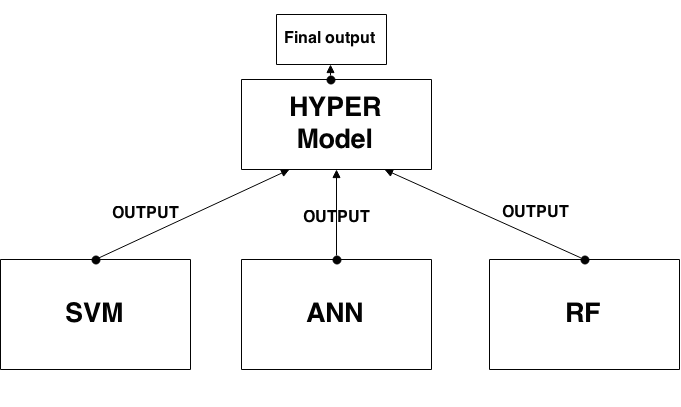
\includegraphics[scale=0.5, keepaspectratio]{Untitled_Diagram.png}
\label{fig:my_label}
\end{figure}


\subsection{Experiment Results}

\subsubsection{Validation Error}

    The Table below is the accuracy rate of model we test on our validation set.
    For support vector machine and  random forest, we conduct n folder validation test, and artificial neural networks we perform batch validation test, which has the same concept of the above method, however it's more efficient when we are doing optimization(mini-batch gradient decent). The reason why we do not use the same method for all models is that different optimization approaches they have have different structures restricting for certain flexibilities. 
    We also present the statistics of our generation process to show whether the generated validation error is a descent proxy for out of sample error.
    

\begin{table}[h]
\centering
\begin{tabular}{|c|l|l|l|}
\hline
\multicolumn{1}{|l|}{Average Validation Errors} & SVM     & ANN    & RF     \\ \hline
Data1                                                  & 23.50\% & 40.0\% & 29.1\% \\ \hline
Data2(PCA, n=20)                                       & 23.75\% & 34.0\% & 27.5\% \\ \hline
Data3(PCA, n=8)                                        & 31.75\% & 2.0\%  & 35.4\% \\ \hline
Data4(PCA, n=20)                                       & 25.5\%  & 40.0\% & 23.6\% \\ \hline
\end{tabular}

\end{table}

    As you can see, the result is frustrating, the errors is some where around 50\% that means our model can not beat the random guess.
    And we next conduct some tests to see what we can improve in next experiment.


\subsubsection{Confusion Mtrices}
What label our model predict wrongly?
\subsection{Feature Selection}
\subsection{Summary for Experiment 1}
1.We should select more meaningful feature to help us to explore the promising features.

2.The frequency of label is too high, and the pattern of label is noisy. We should define the 'answer' more carefully.

3.The feature selection result shows that coil oil price maybe a light of exchange rate prediction.

4. The hourly prediction is merely impossible for economic variables.

5. The result shows that Conditional Restricted Boltzmann machine maybe perform better than the traditional time series process.

\section{Experiment 2}

\subsection{Data description}
We collect the following data from Thomas Routers Data Stream database.
    We divide the factors into different aspects which may affect the exchange rate.


\begin{enumerate}
\item{Stock Market Indice}

\begin{enumerate}
    \item{S&P 500 Index}
    \item{Dow Jons Index}
    \item{Euro stoxx 50 }
    \item{Deutscher Aktienindex}
    \item{France Cotation Assistée en Continu 40}
    \item{NASCOMP}
    \item{Nikki}
\end{enumerate}

\item{Bond Market}
\subitem{}
\subitem{}
\item{Money Supply}
\item{Commodity}

\item{Other Indice}

\end{enumerate}
\newpage
    We describe our data as the market information. 


\subsection{Labeling}

    In Experiment 2 we present two labeling approach. From previous Experiment 1, we know something about that it is very difficult to predict the price movement by economic variables, however it might be result from the factors we select did not contain the crucial information about the price movement, or otherwise from efficient market hypothesis, it is not possible for people gain from historical information under weak form of market efficiency.
    
    Second we construct a equally weighted foreign exchange carry portfolio. From the Experiment 1 we calculate the movement of exchange rate by testing whether the current ask price is higher than the future bid price. The method may result  very noisy labeling pattern, which economic factors cannot catch. To prevent the chaotic pattern we construct a portfolio for our labeling target.
    
    Third we use daily frequency. The lower frequency maybe improve the performance of model.
    
    For label 1 we inherent the method from Experiment 1.The procedure is as follow.
We calculate the daily return of our representative portfolio
if the return is negative we label it as -1 then, positive as +1.

    For label 2, we assume there is impossible for us to predict the daily return movement. So we construct a totally different labeling method. CAPM supports that only systematic risk will be compensated, if CAPM holds the daily return of the market portfolio will explain the daily return. What if we can predict the covariance movement of the portfolio ? Can we beat the market?
    
\subsubsection{Market Correlation Coefficient Matrix}
    We define the market correlation coefficient matrix is the correlation matrix of 7 pairs of currency against GBP. The reason why we use GBP because United Kingdom have higher and more stable interest rate than average country, making interest spread higher. The naive  correlation matrix is calculated as follow.
    $$\rho (x_{i,T},x_{j,T}) = \frac{1}{l}\sum^{T}_{t=T-l}(x_{i,T-t} - \bar{x_{i}})(x_{j,T-t}-\bar{x_{j}})$$
    For our experiment this is totally wrong, and is not a consistent estimator of our market correlation coefficient matrix. What is our target parameter? $\rho(x_{i,t},x_{j,t}) \forall i \not j$ is what we are interested in. The equation above has shown that all we needed is that use past experience to estimate it, however that just show how innocent we are. That means we believe the past experience will happen again, which is not. The newly define market correlation matrix is rewritten as below.
    
    $$\rho (x_{i,T},x_{j,T}) = \frac{1}{l+f}\sum^{T+f}_{t=T-l}(x_{i,T-t} - \bar{x_{i}})(x_{j,T-t}-\bar{x_{j}})$$
    
    This estimator is consistent for market correlation coefficient, however we cannot get at time T, and the idea is somehow connect to local learning. CRBM maybe a promising estimation for the market correlation matrix.
    
\subsubsection{Market Momentum}

We define the market momentum as the distance between the market correlation matrix and the identity matrix. We use euclidean space as our metric space. The different metric space will result different strategy performance. For a baseline we use euclidean space.
    $$d(\rho(x_{t}), \mathbf(I))$$
    There are some economics features about market momentum. It is a proxy for risk in risk out.
    
\begin{figure}
\caption{Market Momentum Histogram}
\centering
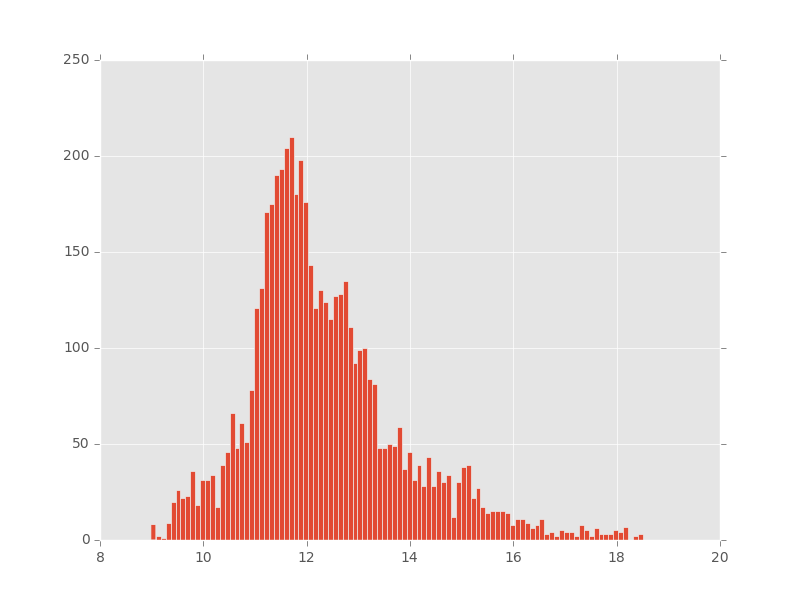
\includegraphics[scale=0.5, keepaspectratio]{market_momentum.png}
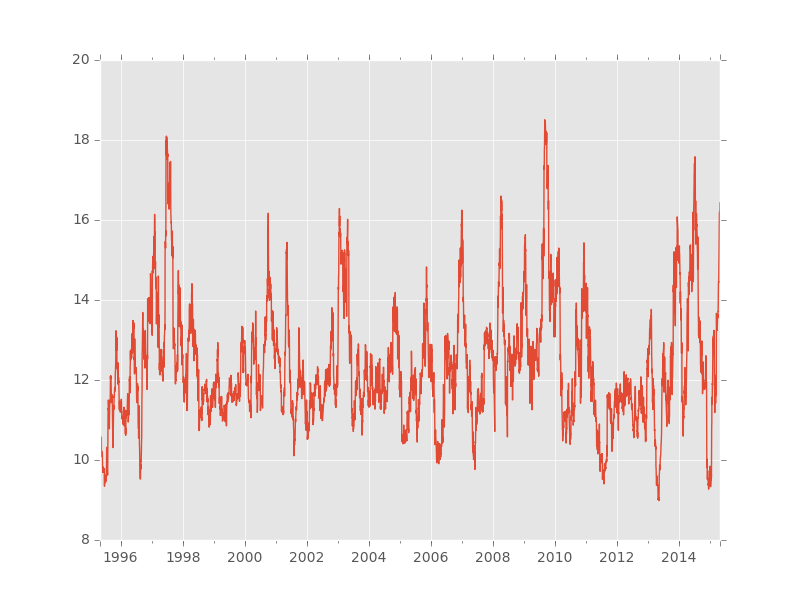
\includegraphics[scale=0.5, keepaspectratio]{historial_market_momentum.png}
\label{fig:my_label}
\end{figure}


\subsubsection{Mixing the whole idea}
    Our Experiment2 present a new designed labeling techniques, the procedure is as follow. We calculate the market momentum, then if the market momentum is greater than it's 25\% quantile  than we label as 1 others we label as 0.
    Is it valid for us to use quantile as a threshold? We found that the time-variant distribution of market momentum is very stable.

\subsection{Data Pre-process}
    Corresponding to the previous experiment, we conduct the same data pre-process methods.  
    
\begin{table}[h]
\centering
\begin{tabular}{|l|l|l|l|l|}
\hline
      & Data              & Process1    & Process2      & Process2 \\ \hline
Data1 & With Lag-terms    & None        & None          & None     \\ \hline
Data2 & With Lag-terms    & PCA         & None          & None     \\ \hline
Data3 & Without Lag-terms & Standardize & 1-layer CRBM(6-Delay)  & PCA      \\ \hline
Data4 & Without Lag-terms & PCA         & None          & None     \\ \hline
\end{tabular}
\end{table}



\subsection{Result}

The training result is shown below.
\subsubsection{Validation Error}

\begin{table}[h]
\centering
\begin{tabular}{|l|l|l|l|l|}
\hline
      & Data              & Process1    & Process2      & Process2 \\ \hline
Data1 & With Lag-terms    & None        & None          & None     \\ \hline
Data2 & With Lag-terms    & PCA         & None          & None     \\ \hline
Data3 & Without Lag-terms & Standardize & 1-layer CRBM(6-Delay)  & PCA      \\ \hline
Data4 & Without Lag-terms & PCA         & None          & None     \\ \hline
\end{tabular}
\end{table}
    The result is very promising. It is possible for us to predict the future market momentum. 

    There are few interesting thing has shown on the result. As we use CRBM as an autoencoder of our data set the error rate is higher than the others data sets. There are few explanation of the difference. 
    First, the historical path of the economics variables has no information of the future market momentum. 
    Second is the CRBM is under fitting, as the data set 1 has reached to $ $ error rate, under the hypothesis that historical path is very important for making prediction on market momentum, it is less likely to have a low accuracy rate of the CRBM than the others discriminative model.

    Since our experiment is extremely successful. This might impose that human portfolio mangers may be defeated by the machine experts which are designed by machine learning experts. The intuition behind the label which predict by the machine can be seen as a risk metric.


\subsection{Test set}


\subsubsection{Currency portfolio}
We choose 7 pairs of currency to form our equally-weighted portfolio.
First benchmark is that we just hold the portfolio for long term.
Second benchmark is the VIX trading strategy, if the VIX index fall below its $0.25$ quantile, we long the equally-weighted portfolio, vise versa.
\subsubsection{Forex carry portfolio}


We also apply the label in our simple strategy. If the model predicts 1 which means that that the market momentum is strengthen by the current market conduction, we would have a long position on risk free rate. If the model predicts 0 then we hold the equally-weighted portfolio. The accumulated sum of the daily return is illustrated in graph. We do not present the further test on our strategy because that is not our focus in this paper.

\subsection{Conclusion}

\subsection{Further Works}
Label serve as a new risk metric{predict daily currency movement}
Test the strategy performance.
Different markets.
Correlation coefficient matrix prediction and estimation.
Optimal portfolio with conditional predictability.
Testing CAPM.
Testing Consumption-based asset pricing model.


 % Experimental Setup

%\input{Chapters/Chapter4} % Experiment 1

%\input{Chapters/Chapter5} % Experiment 2

%\input{Chapters/Chapter6} % Results and Discussion

%\input{Chapters/Chapter7} % Conclusion

%% ----------------------------------------------------------------
% Now begin the Appendices, including them as separate files

\addtocontents{toc}{\vspace{2em}} % Add a gap in the Contents, for aesthetics

\appendix % Cue to tell LaTeX that the following 'chapters' are Appendices

\chapter{An Appendix}

\begin{figure}
\caption{Time Series Figures}
\centering
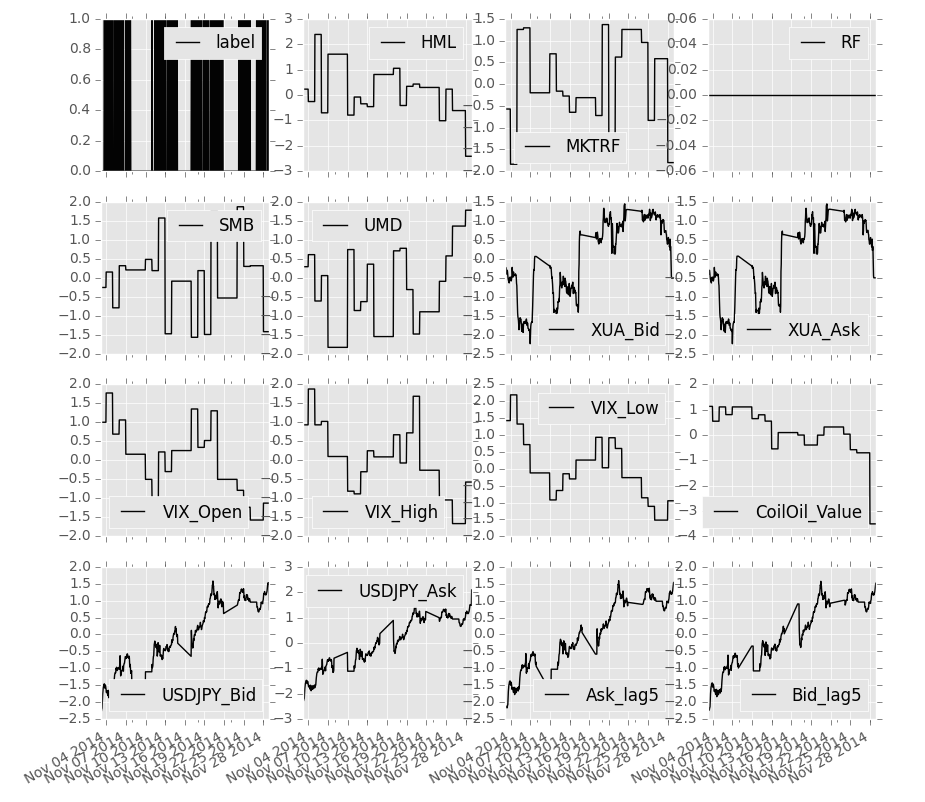
\includegraphics[width=\textwidth,height=\textheight,keepaspectratio]{data_ver3_descrip.png}

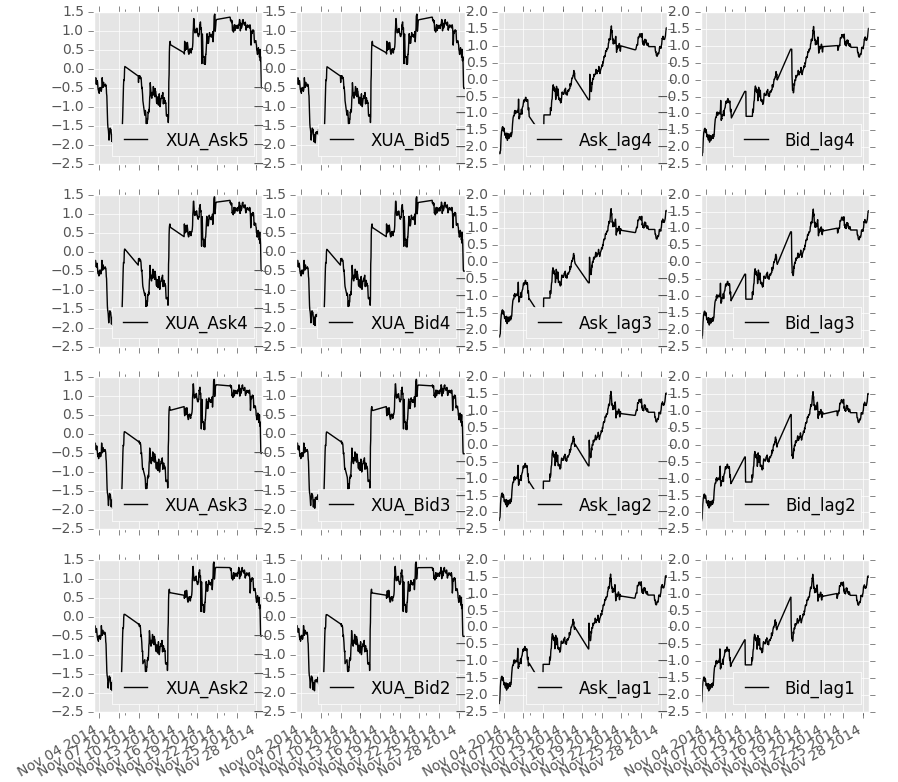
\includegraphics[width=\textwidth,height=\textheight,keepaspectratio]{data_ver3_descrip2.png}

\label{fig:my_label}
\end{figure}	% Appendix Title

%\input{Appendices/AppendixB} % Appendix Title

%\input{Appendices/AppendixC} % Appendix Title

\addtocontents{toc}{\vspace{2em}}  % Add a gap in the Contents, for aesthetics
\backmatter

%% ----------------------------------------------------------------
\label{Bibliography}
\lhead{\emph{Bibliography}}  % Change the left side page header to "Bibliography"
\bibliographystyle{unsrtnat}  % Use the "unsrtnat" BibTeX style for formatting the Bibliography
\bibliography{Bibliography}  % The references (bibliography) information are stored in the file named "Bibliography.bib"

\end{document}  % The End
%% ----------------------------------------------------------------